\documentclass[11pt,a4paper,titlepage]{article}
\usepackage[brazil]{babel}
\usepackage[utf8]{inputenc}
\usepackage[T1]{fontenc}

\newcommand{\titulo}{\textit{Relatório I - Unidade Lógica Aritmética}}

\newcommand{\cabecalho}{\textit{Relatório I}}

\usepackage{fancyhdr}
\usepackage{indentfirst}
\usepackage{setspace}
\usepackage{graphicx,url}
%\usepackage{color,colortbl}
\usepackage{amsmath}
\usepackage{amssymb}
\usepackage{amsthm}
\usepackage{wrapfig}
\usepackage{times}
\usepackage{hyphenat}
\usepackage{ae}
\usepackage{algorithm}
\usepackage[sort,numbers]{natbib}
%package to insert codes
\usepackage{listings}
\usepackage{mips}
\usepackage{tabularx}
\usepackage{makecell}
%appendix
\usepackage[titletoc,toc,page]{appendix}
\renewcommand{\appendixtocname}{Apêndices}
\renewcommand{\appendixpagename}{Apêndices}

% the following is needed for syntax highlighting
\usepackage{color}

\definecolor{dkgreen}{rgb}{0,0.6,0}
\definecolor{gray}{rgb}{0.5,0.5,0.5}
\definecolor{mauve}{rgb}{0.58,0,0.82}

\lstset{ %código assembly
  language=[mips]Assembler,       % the language of the code
  basicstyle=\footnotesize,       % the size of the fonts that are used for the code
  numbers=left,                   % where to put the line-numbers
  numberstyle=\tiny\color{gray},  % the style that is used for the line-numbers
  stepnumber=1,                   % the step between two line-numbers. If it's 1, each line 
                                  % will be numbered
  numbersep=5pt,                  % how far the line-numbers are from the code
  backgroundcolor=\color{white},  % choose the background color. You must add \usepackage{color}
  showspaces=false,               % show spaces adding particular underscores
  showstringspaces=false,         % underline spaces within strings
  showtabs=false,                 % show tabs within strings adding particular underscores
  frame=single,                   % adds a frame around the code
  rulecolor=\color{black},        % if not set, the frame-color may be changed on line-breaks within not-black text (e.g. commens (green here))
  tabsize=4,                      % sets default tabsize to 2 spaces
  captionpos=b,                   % sets the caption-position to bottom
  breaklines=true,                % sets automatic line breaking
  breakatwhitespace=false,        % sets if automatic breaks should only happen at whitespace
  title=\lstname,                 % show the filename of files included with \lstinputlisting;
                                  % also try caption instead of title
  keywordstyle=\color{blue},          % keyword style
  commentstyle=\color{dkgreen},       % comment style
  stringstyle=\color{mauve},         % string literal style
  escapeinside={\%*}{*)},            % if you want to add a comment within your code
  morekeywords={*,...}               % if you want to add more keywords to the set
}
\usepackage{xcolor}
\definecolor{vgreen}{RGB}{104,180,104}
\definecolor{vblue}{RGB}{49,49,255}
\definecolor{vorange}{RGB}{255,143,102}
%mostrar código do verilog
\lstdefinestyle{verilog-style}
{
    language=Verilog,
    basicstyle=\small\ttfamily,
    keywordstyle=\color{vblue},
    identifierstyle=\color{black},
    commentstyle=\color{vgreen},
    numbers=left,
    numberstyle=\tiny\color{black},
    numbersep=10pt,
    tabsize=8,
    moredelim=*[s][\colorIndex]{[}{]},
    literate=*{:}{:}1
}

\makeatletter
\newcommand*\@lbracket{[}
\newcommand*\@rbracket{]}
\newcommand*\@colon{:}
\newcommand*\colorIndex{%
    \edef\@temp{\the\lst@token}%
    \ifx\@temp\@lbracket \color{black}%
    \else\ifx\@temp\@rbracket \color{black}%
    \else\ifx\@temp\@colon \color{black}%
    \else \color{vorange}%
    \fi\fi\fi
}
\makeatother

\usepackage{trace}

% Criar figura dividida em subfiguras
\usepackage{subfigure}

\usepackage{subfig}
\usepackage{ae}
\usepackage{aecompl}

\usepackage{multirow}
%\usepackage{epstopdf}

\pagestyle{fancy}

\setlength{\evensidemargin}{0.0in}
\setlength{\oddsidemargin}{0.0in}
\setlength{\textwidth}{6.6in}
\setlength{\textheight}{1.06\textheight}

\lhead{}
\chead{}
\rhead{\footnotesize{\textsc{\cabecalho}}}
\lfoot{\footnotesize{Guilherme Batista Santos, Iuri Silva Castro, João Mateus de Freitas Veneroso, Ricardo Pagoto Marinho}}
\cfoot{}
\rfoot{\footnotesize{\thepage}}
\setlength{\headwidth}{\textwidth}
\renewcommand{\headrulewidth}{0.4pt}
\renewcommand{\footrulewidth}{0.4pt}
\renewcommand{\baselinestretch}{0.90}

%\hyphenation{ ca-rac-te-ri-zan-do--se }

\begin{document}

\begin{titlepage}
\begin{center}

\begin{large}
Universidade Federal de Minas Gerais\\
Instituto de Ciências Exatas\\
Departamento de Ciência da Computação\\
\end{large}

\vspace{20mm}

\begin{Large}
DCC819 - Arquitetura de Computadores
\end{Large}

\vspace{20mm}

\begin{LARGE}
\titulo
\end{LARGE}


\vspace{30mm}

\begin{Large}
\begin{center}
Guilherme Batista Santos\\ Iuri Silva Castro\\ João Mateus de Freitas Veneroso\\ Ricardo Pagoto Marinho \\
\end{center}
\end{Large}


\vspace{60mm}

{\sc Belo Horizonte - MG}

{\sc \today}
%{\sc 05 de Maro de 2012}

%\vspace{10mm}
\end{center}
\end{titlepage}


\section{Introdução}\label{sec:intro}

A Unidade Lógica Aritmética, ou \textit{ULA}, é um circuito digital responsável por realizar operações lógicas e aritméticas no microprocessador, como por exemplo, operações de adição, subtração, deslocamentos lógicos, operações lógicas \textit{and} e \textit{or}. A Figura~\ref{fig:ula} abaixo mostra a forma geral de uma ULA.

\begin{figure}[h]
\centering

\includegraphics[scale=0.8]{images/ALU_symbol.png}
\caption{Unidade Lógica Aritmética.}
\label{fig:ula}
\end{figure}

A unidade possui duas entradas e uma saída de dados,~\textit{A}, \textit{B} e~\textit{R} respectivamente, além de entradas e saídas de sinais de controle,~\textit{F} e~\textit{D}. As entradas \textit{A} e~\textit{B} são conhecidas como \textit{operandos}, valores em que a unidade executará a operação designada. O resultado da operação será dado em \textit{R}. Os sinais entrada de controle \textit{F} indicam a unidade, por exemplo, qual operação deverá ser feita, e os sinais de saída \textit{D} são utilizados, por exemplo, para indicar o estado do resultado da operação como indicação de valor zero, negativo ou se houve~\textit{overflow} na operação.

Propõe-se, para esse trabalho, implementar uma Unidade Lógica Aritmética capaz de realizar operações específicas. Será utilizada a linguagem de descrição de hardware \textit{Verilog HDL} e a plataforma \textit{Quartus II} para a implementação. O simulador \textit{ModelSim} será utilizado para auxiliar na verificação e testes da implementação. Testes físicos serão feitos no módulo de prototipação Altera DE2.

Futuramente, a ULA descrita neste trabalho será integrada como parte de um microprocessador.

\section{Descrição}\label{sec:desc}

Deseja-se que o microprocessador seja capaz de executar as instruções conforme a Tabela ~\ref{tab:ULA}. As instruções são de 16-bits e trabalham com registradores de 16-bits e imediatos absolutos de 4-bits. Cada instrução possui um código de operação de 4-bits, código do registrador de destino \$s4 de 4-bits, código do registrador \$s3 ou o imediato absoluto de 4-bits e o código do registrador operando \$s2 de 4-bits.

\begin{table}[h]
\centering
\begin{tabular}{| c | c | c | l |}
\hline
Código & Instrução & Operação & Descrição\\
\hline
0 & ADD \$s4,\$s3,\$s2 & \$s4 = \$s2 + \$s3 & \makecell{Adição entre \\ registros}\\
\hline
1 & SUB \$s4,\$s3,\$s2 & \$s4 = \$s3 - \$s2 & \makecell{Subtração entre \\ registros} \\
\hline
2 & SLTI \$s4,imm,\$s2 & \$s2 > imm ? \$s4 = 1 : \$s4 = 0 & \makecell{Comparação entre \\ registro e imediato }\\
\hline
3 & AND \$s4,\$s3,\$s2 & \$s4 = \$s2 and \$s3 & \makecell{\textit{AND} lógico \\ com dois registros}\\
\hline
4 & OR \$s4,\$s3,\$s2 &  \$s4 = \$s2 or \$s3 & \makecell{\textit{OR} lógico \\ com dois registros}\\
\hline
5 & XOR \$s4,\$s3,\$s2 &  \$s4 = \$s2 xor \$s3 & \makecell{\textit{XOR} lógico \\ com dois registros}\\
\hline
6 & ANDI \$s4,imm,\$s2 & \$s4 = \$s2 and imm & \makecell{\textit{AND} lógico com \\ um registro e um imediato}\\
\hline
7 & ORI \$s4,imm,\$s2 & \$s4 = \$s2 or imm & \makecell{\textit{OR} lógico com \\ um registro e um imediato} \\
\hline
8 & XORI \$s4,imm,\$s2 & \$s4 = \$s2 xor imm & \makecell{\textit{XOR} lógico com \\ um registro e um imediato} \\
\hline
9 & ADDI \$s4,imm,\$s2 & \$s4 = \$s2 + imm & \makecell{Adição entre \\ registro e um imediato}\\
\hline
10 & SUBI \$s4,imm,\$s2 & \$s4 = \$s2 - imm & \makecell{Subtração entre \\ registro e um imediato}\\
\hline
\end{tabular}
\caption{Descrição das instruções requisitadas.}
\label{tab:ULA}
\end{table}
\captionsetup{font={footnotesize,rm},justification=centering,labelsep=period}

Observa-se que há instruções que trabalham com operandos registro-registro e operandos registro-imediato. Tais operações não são distinguidas pela ULA, indicando apenas se um dos operandos virá do banco de registradores ou da própria instrução. A unidade precisa apenas executar as operações de adição, subtração, comparação, E, OU e OU-EXCLUSIVO, deixando a parte de decisão de operandos para a unidade de decodificação.

Observa-se também que para a instrução de subtração, em que a posição dos operandos altera o resultado, a subtração entre registros e a subtração entre registro-imediato tem a forma \$s4 = \$s3 - \$s2 e \$s4 = \$s2 - imm. Para tornar a ULA genérica e diminuir a complexidade, optou-se pela modificação da instrução de subtração entre registros, ficando da forma \$s4 = \$s2 - \$s3.

Sinais de indicação de características do resultado da operação são desejáveis, assim opta-se por um registro de indicadores de \textit{zero}, \textit{negativo} e \textit{overflow}, conforme a Tabela \ref{tab:flags} abaixo, sendo esse registro atualizado a cada operação da unidade.

\begin{table}[h]
\centering
\begin{tabular}{| c | c |}
\hline
Índice & Sinal\\
\hline
0 & \textit{Overflow}\\
\hline
1 & Negativo \\
\hline
2 & Zero\\
\hline
\end{tabular}
\caption{Sinais de saída da ULA.}
\label{tab:flags}
\end{table}
\captionsetup{font={footnotesize,rm},justification=centering,labelsep=period}%

Definido as instruções, parte-se para a implementação.

\section{Implementação}

Necessita-se, além da ULA, de implementar unidades auxiliares, como o banco de registradores e a unidade de decodificação, que dão suporte ao funcionamento da ULA. Implementa-se também uma unidade de controle para comandar a execução das instruções propostas. As seções seguintes descrevem o funcionamento e a implementação das unidades.

\subsection{Banco de registradores}\label{subsec:imp-br}

O banco de registradores é utilizado para fazer o armazenamento temporário de valores que serão utilizados e escritos pela ULA. Implementou-se um banco de registradores com em 16 registradores de 16-bits cada. A Figura \ref{fig:blocoregbank} mostra os sinais de entrada e saída do módulo.

\begin{figure}[h]
\centering
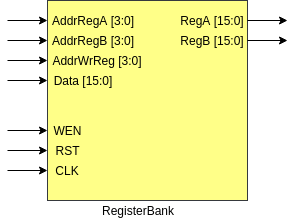
\includegraphics[scale=0.5]{images/RegisterBank.png}
\caption{Bloco do Banco de Registradores.}
\label{fig:blocoregbank}
\end{figure}

O módulo possui três entradas de 4-bits para endereços de registros, sendo dois endereços para leitura dos registros A e B (\textit{AddrRegA} e \textit{AddrRegB}), com os dados de leitura apresentados em \textit{RegA} e \textit{RegB}, e um endereço (\textit{AddrWriteReg}) para escrita do valor de entrada (\textit{Data}). Há três sinais de controle, sendo:

\begin{itemize}
\item WEN (\textit{Write Enable}): Indica a operação do banco (leitura ou escrita). Ele será escrito, caso WEN=1 e lido caso WEN=0;
\item RST (\textit{Reset}): Faz o \textit{reset} do banco, zerando os valores de todos os registros;
\item CLK (\textit{Clock}): Utilizado para sincronização e execução.
\end{itemize}

Para a utilização correta do módulo primeiro deve-se definir qual será a operação a ser realizada (leitura ou escrita) e o devido sinal deve ser colocado em WEN. Os endereços dos registros devem ser definidos e, em seguida, deve-se fazer uma transição do sinal de relógio (CLK) para que a operação seja executada.

O sinal de \textit{reset} (RST) deve ser mantido em nível lógico baixo durante toda a execução. Ele é utilizado apenas para a inicialização do banco de registros.

\subsection{ULA}\label{subsec:imp-ula}

O módulo desenvolvido possui 5 entradas e duas saídas: \textit{OpA}, \textit{OpB}, \textit{Op}, \textit{RST}, \textit{CLK}, \textit{Res} e \textit{FlagReg} respectivamente. A Figura \ref{fig:blocoula} mostra os sinais de entrada e saída do módulo.

\begin{figure}[h]
\centering
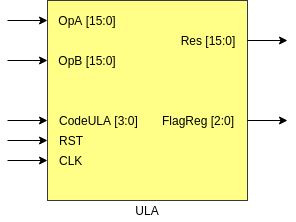
\includegraphics[scale=0.5]{images/ULA_diag.png}
\caption{Bloco da ULA.}
\label{fig:blocoula}
\end{figure}

As entradas \textit{OpA} e \textit{OpB} representam os operandos de 16-bits \textit{A} e \textit{B} a serem utilizados na operação. A entrada \textit{CodeULA} de 4-btis indica qual operação a ser executada, como adição, subtração, etc., conforme a Tabela \ref{tab:imp} abaixo. As saídas \textit{Res} de 16-bits e \textit{FlagReg} de 3-bits indicam, respectivamente, o resultado da operação e o estado do resultado.

Conforme descrito anteriormente, não há destinção, por parta da ULA, se o operando é um imediato ou um registro. Assim, cria-se a partir das instruções desejadas na Tabela \ref{tab:ULA}, uma ULA com as seguintes instruções genéricas:

\begin{table}[h]
\centering
\begin{tabular}{| c | c |}
\hline
Código  & Operação \\
\hline
0000 & Adição\\
\hline
0001 & Subtração\\
\hline
0010 & Comparação\\
\hline
0011 & \textit{AND} lógico\\
\hline
0100 & \textit{OR} lógico\\
\hline
0101 & \textit{XOR} lógico\\
\hline
\end{tabular}
\caption{Descrição das operações implementadas.}
\label{tab:imp}
\end{table}
\captionsetup{font={footnotesize,rm},justification=centering,labelsep=period}%

Optou-se por implementar uma ALU síncrona, utilizando o passo do relógio (CLK) para orientar sua execução. Assim, depois de selecionados os operandos e a operação a ser executada, deve-se fazer uma transição no sinal de clock para que a operação seja realizada. O sinal de reset (RST) é utilizado apenas para limpar o registro de estados \textit{FlagReg} e deve ser mantido em nível lógico baixo durante a execução.

Todas as operações da ALU modificam todos os campos do registro de estados \textit{FlagReg}.

\subsection{Decodificador}\label{subsec:decode}

O decodificador é responsável por receber a instrução e fazer a seleção correta dos operandos e da operação na ULA. Ele recebe a instrução de 16-bits na forma \textit{INSTR DST, IMM|REGB, REGA}, onde

\begin{itemize}
\item \textit{INSTR} (4-bit): Código da instrução, conforme a Tabela \ref{tab:ULA};
\item \textit{DST} (4-bit): Endereço do registrador de destino;
\item \textit{IMM/REGB} (4-bit): Endereço do registrador operando (RegB) ou imediato absoluto;
\item \textit{REGA} (4-bit): Endereço do segundo registrador operando (RegA).
\end{itemize}

\begin{figure}[h]
\centering
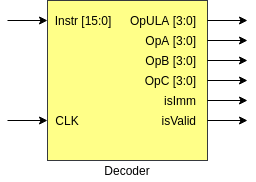
\includegraphics[scale=0.5]{images/Decoder.png}
\caption{Bloco do Decodificador.}
\label{fig:blocodecoder}
\end{figure}

O módulo retorna, em suas saídas, os endereços dos operandos (\textit{OpC}, \textit{OpA} e \textit{OpB}), a operação a ser executada pela ALU (\textit{OpALU}), a indicação se o operando B é um registro ou um imediato (\textit{isImm}) e indica se a instrução é válida ou não (\textit{isValid}).

A sincronia é feita através do sinal de \textit{clock}. Assim, a cada transição do sinal verifica-se o código da instrução, altera-se os sinais de \textit{isImm} e \textit{isValid}, ajusta os endereços dos operandos e a operação da ALU. Os códigos da \textit{OpALU} seguem a Tabela \ref{tab:imp}.

\section{Integração}

Após a implementação dos módulos, faz-se a integração dos mesmos para testar o funcionamento da ULA e suas respostas as instruções. É necessário implementar uma pequena unidade de controle com uma máquina de estados para gerenciar o fluxo dos dados no microprocessador.

Fluxo: Decodificador -> Banco de Registradores -> ULA -> Banco de Registradores


-- REVISADO ATÉ AQUI --


Por último, descreveremos como implementamos o estágio do caminho de dados para saber o que fazer em cada \textit{clock}.

Os estágios foram implementados como uma máquina de estados, ou seja, a cada subida de \textit{clock}, mudamos de estado e fazemos um estágio do caminho de dados.
Inicialmente, a máquina começa no estado de \textit{Halt} esperando alguma ação.
O estado muda assim que o módulo recebe um sinal de \textit{START}.
Quando o sinal chega, a máquina decodifica a instrução no decodificador.
O próximo passo é ir no bando de registradores e buscar os valores requisitados pela instrução.
Após a busca, a instrução é executada na ALU e então, o resultado é escrito no banco de registradores.
Depois de escrever o resultado, a máquina volta ao estado inicial de \textit{HALT} esperando a próxima instrução.


Como dito anteriormente, a ULA implementada deve ser capaz de realizar 11 operações diferentes.
Observe que é possível, além de fazer operações com registradores, realizar operações com imediatos, \textit{i.e.}, números absolutos.
Esses números devem possuir 4 bits de largura.

As duas \textit{flags} indicam se a operação será realizada com um imediato e se ela é válida, ou seja, foi implementada pela ALU.
A \textit{flag isImm} que indica para o multiplexador qual entrada a ALU deverá receber, se do banco de registradores ou se é um imediato, logo, essa \textit{flag} serve como entrada de seleção do multiplexador, descrito na próxima subseção.


A saída \textit{RegA} do banco de registradores se conecta à entrada \textit{OpA} do módulo da ULA, enquanto a saída \textit{RegB}, se conecta à entrada \textit{OpB} do módulo da ULA.
Lembrando que essa entrada da ULA pode ser um imediato, a decisão de pegar a saída do banco de registradores ou o imediato segue como descrito na Seção~\ref{subsec:mux}.



\subsection{Multiplexador}\label{subsec:mux}

O multiplexador implementado tem como entrada dois valores \textit{A} e \textit{B} além de um seletor \textit{SEL}.
A saída é o resultado da seleção do multiplexador: \textit{S}.

Caso o valor em \textit{SEL} seja 0, a saída é o valor de um registrador, indicado pela entrada \textit{A}.
Caso o valor seja 1, então o valor é um imediato estendido em 12 bits, vindo da entrada \textit{B}.
Com isso, a ALU fica genérica o suficiente para sua lógica não se preocupar com operações que recebam imediato ou valor de registrador.
É importante frisar que o multiplexador é responsável apenas pela entrada \textit{B} da Figura~\ref{fig:ula}.
Como explicado anteriormente, essa entrada que, caso a instrução requisite, recebe um imediato ao invés de um registrador.




\subsection{Prototipação}\label{subsec:prot}

A FPGA utilizada para a prototipação possui 4 botões para que possamos inserir dados e realizar as operações, 16 \textit{switches} para informar o valor dos dados inseridos e 8 \textit{displays} que mostram o valor dos dados.
Cada \textit{switch} possui dois estados: \textit{cima} e \textit{baixo}.
Quando um \textit{switch} está no estado \textit{cima}, ele possui valor 1, e quando está no estado \textit{baixo}, ele possui valor 0.
Desta forma, cada \textit{switch} se comporta com 1 bit do dado.

Quando o botão de nome \textit{KEY0} for apertado, os \textit{displays HEX7} e \textit{HEX6} mostram o valor no conjunto de \textit{switches} \textit{SW8} a \textit{SW11} (4 bits) e os \textit{displays HEX5} e \textit{HEX4} mostram o valor no conjunto de \textit{switches} \textit{SW4} a \textit{SW7} (4 bits).
Desta forma, é possível visualizar os valores passados para a placa.

Se apertarmos o botão \textit{KEY3}, os \textit{switches} serão interpretados como uma instrução completa, ou seja, com código da operação e operandos de entrada e saída, sendo que o \textit{switch SW0} é o menos significativo enquanto o \textit{SW15} o mais significativo.
Assim, cada instrução possui 16 bits, como especificado no documento.
O conjunto de \textit{switches} \textit{SW0} a \textit{SW3} indica a entrada \textit{A} e do \textit{switch SW4} ao \textit{SW7}, a entrada \textit{B} da Figura~\ref{fig:ula}.
Lembrando que a entrada \textit{B} pode ser um imediato.
Já o conjunto de \textit{switches SW8} a \textit{SW11} indica a saída do resultado (saída R na Figura~\ref{fig:ula}), enquanto os \textit{switches SW12} a \textit{SW15} indicam a operação a ser realizada, \textit{i.e.}, o código da operação.

A Figura~\ref{fig:fpga} mostra a divisão na placa.

\begin{figure}[h]
\centering
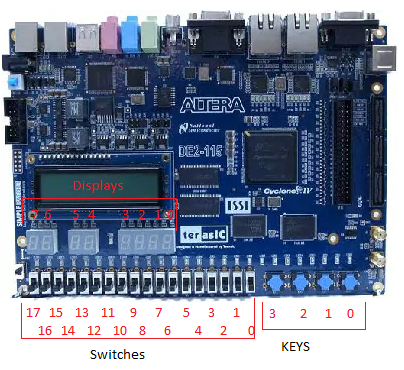
\includegraphics[]{images/FPGA.png}
\caption{Módulo Altera DE2.}
\label{fig:fpga}
\end{figure}


\section{Experimentos}

\begin{table}[t]
\centering
\begin{tabular}{|l|l|l|l|l|l|l|}
\hline
Instrução & Operando A & Operando B & Resultado & O & N & Z \\
\hline
ADD & 0011 1111 1111 1111 & 0100 0000 0000 0000 & 0111 1111 1111 1111 & 0 & 0 & 0 \\
ADD & 0100 0000 0000 0000 & 0100 0000 0000 0000 & 1000 0000 0000 0000 & 1 & 1 & 0 \\
ADD & 0000 0000 0000 0000 & 0000 0000 0000 0000 & 0000 0000 0000 0000 & 0 & 0 & 1 \\
ADD & 0010 0000 0000 0000 & 1100 0000 0000 0000 & 1110 0000 0000 0000 & 0 & 1 & 0 \\
SUB & 0100 0000 0000 0000 & 0011 1111 1111 1111 & 0000 0000 0000 0001 & 0 & 0 & 0 \\
SUB & 0011 1111 1111 1111 & 0100 0000 0000 0000 & 1111 1111 1111 1111 & 0 & 1 & 0 \\
SLT & 0100 0000 0000 0000 & 0000 0000 0000 0000 & 0000 0000 0000 0001 & 0 & 0 & 0 \\
SLT & 0000 0000 0000 0000 & 0100 0000 0000 0000 & 0000 0000 0000 0000 & 0 & 0 & 1 \\
AND & 0111 1111 1111 1111 & 0011 1111 1111 1111 & 0011 1111 1111 1111 & 0 & 0 & 0 \\
OR  & 0000 0000 1111 1111 & 1111 1111 0000 0000 & 1111 1111 1111 1111 & 0 & 1 & 0 \\
XOR & 0101 0101 0101 0101 & 0010 1010 1010 1010 & 0111 1111 1111 1111 & 0 & 0 & 0 \\
\hline

\end{tabular}
\caption{Experimentos.}
\label{tab:experiments}
\end{table}
\captionsetup{font={footnotesize,rm},justification=centering,labelsep=period}%

Alguns experimentos foram realizados com o intuito de testar as funcionalidades da Unida Lógica Aritmética
implementada em Verilog HDL. Observe que a ULA não distingue operações com registradores e imediatos, uma 
vez que os operandos A e B são tratados pelo módulo \textit{Decoder} e transformados em sua representação 
númerica de 16 bits antes de serem encaminhados à ULA. Durante o estágio de decodificação, os valores dos 
registradores enderaçados pela instrução são lidos do banco de registradores e um \textit{padding} de 12 
bits é concatenado ao valor dos operandos imediatos. Dessa forma, a ULA precisa executar apenas seis tipos 
de instruções: ADD, SUB, SLT, AND, OR e XOR. 

A tabela \ref{tab:experiments} descreve os resultados de onze  instruções e o valor das \textit{flags} da 
ULA após o término de cada operação. As colunas O, N e Z se referem respectivamente às flags \textit{Overflow}, 
\textit{Negative} e \textit{Zero}. Os experimentos também estão descritos no formato de um \textit{Test Bench} 
implementado no arquivo "\textit{ULA.v}".

Para realizar os experimentos na placa, um dos \textit{switches} foi utilizado como chave para que a instrução fosse executada.
Como o \textit{clock} da placa é de 50 MHz, sempre que o botão \textit{Key3} era apertado, a instrução era executada 50 milhões de vezes, o que inviabilizava a visualização correta do resultado.
Para superar este problema, o \textit{switch} 17 foi utilizado para que a instrução executasse apenas uma vez quando ele estivesse com o valor 1.
Após a execução da instrução e a consequente visualização do resultado, temos que reiniciar o \textit{switch}, ou seja, colocar ele no valor 0 e novamente no valor 1.
Com isso, garantimos que a instrução é executada apenas uma vez, com o custo de ter que reiniciar o \textit{switch} toda vez que fomos executar uma instrução novamente, mesmo se for a mesma operação com os mesmos valores de entrada e saída.


%\begin{appendices}
%	\chapter{Módulo ULA}
%	\label{app:ULA}
%	\begin{lstlisting}[style={verilog-style}]
%module ULA (OpA, OpB, Res, Op, FlagReg, CLK, RST);
%
%	input CLK, RST;
%	input [3:0] Op;
%	input [15:0] OpA, OpB;
%	output reg [15:0] Res;
%	output reg [2:0] FlagReg;		// [Z N C]: Z=Zero; N=Neg; C=Carry/Overflow
%	
%	wire [15:0] invOpB;
%	assign invOpB = ~OpB + 16'd1;
%
%	parameter InsADD = 4'b0000;	// ADD	Res = OpA + OpB
%	parameter InsSUB = 4'b0001;	// SUB	Res = OpA - OpB
%	parameter InsSLT = 4'b0010;	// SLTI	Res = (OpA > OpB) ? 1 : 0
%	parameter InsAND = 4'b0011;	// AND 	Res = OpA & OpB
%	parameter InsOR =  4'b0100;	// OR 	Res = OpA | OpB
%	parameter InsXOR = 4'b0101;	// XOR 	Res = OpA ^ OpB
%	
%	parameter OverflowFlag	= 0;
%	parameter NegFlag 		= 1;
%	parameter ZeroFlag		= 2;
%	
%	always @(posedge CLK) begin
%	 if (RST) begin
%	  FlagReg = 3'b000;
%	 end
%	 else begin
%	  case (Op)
%	   InsADD: begin			
%	    Res = OpA + OpB;
%					
%	    /* Zero check */
%	    if (Res == 0)
%		 FlagReg[ZeroFlag] = 1'b1;
%	    else
%	     FlagReg[ZeroFlag] = 1'b0;
%	    /* Overflow check */
%	    FlagReg[OverflowFlag] = (OpA[15] & OpB[15] & ~Res[15]) | (~OpA[15] & ~OpB[15] & Res[15]);
%	    /* Negative check */
%	    FlagReg[NegFlag] = Res[15];
%	   end
%	   InsSUB: begin			
%	    Res = OpA + invOpB;
%	    /* Zero check */
%	    if (Res == 0)
%	     FlagReg[ZeroFlag] = 1'b1;
%	    else
%	     FlagReg[ZeroFlag] = 1'b0;
%	    /* Overflow check */
%	    FlagReg[OverflowFlag] = (OpA[15] & invOpB[15] & ~Res[15]) | (~OpA[15] & ~invOpB[15] & Res[15]);
%	    /* Negative check */
%	    FlagReg[NegFlag] = Res[15];
%	   end
%	   InsSLT: begin
%	    if (OpA > OpB)
%	     Res = 16'd1;
%	    else
%	     Res = 16'd0;
%	    /* Zero check */
%	    if (Res == 0)
%	     FlagReg[ZeroFlag] = 1'b1;
%	    else
%	     FlagReg[ZeroFlag] = 1'b0;
%	    /* Overflow check */
%	    FlagReg[OverflowFlag] = (OpA[15] & OpB[15] & ~Res[15]) | (~OpA[15] & ~OpB[15] & Res[15]);
%	    /* Negative check */
%	    FlagReg[NegFlag] = Res[15];
%	   end
%	   InsAND: begin			
%	    Res = OpA & OpB;
%	    /* Zero check */
%	    if (Res == 0)
%	     FlagReg[ZeroFlag] = 1'b1;
%	    else
%	     FlagReg[ZeroFlag] = 1'b0;
%	    /* Overflow check */
%	    FlagReg[OverflowFlag] = (OpA[15] & OpB[15] & ~Res[15]) | (~OpA[15] & ~OpB[15] & Res[15]);
%	    /* Negative check */
%	    FlagReg[NegFlag] = Res[15];
%	   end
%	   InsOR: begin			
%	    Res = OpA | OpB;
%	    /* Zero check */
%	    if (Res == 0)
%	     FlagReg[ZeroFlag] = 1'b1;
%	    else
%	     FlagReg[ZeroFlag] = 1'b0;
%	    /* Overflow check */
%	    FlagReg[OverflowFlag] = (OpA[15] & OpB[15] & ~Res[15]) | (~OpA[15] & ~OpB[15] & Res[15]);
%	    /* Negative check */
%	    FlagReg[NegFlag] = Res[15];
%	   end
%	   InsXOR: begin			
%	    Res = OpA ^ OpB;
%	    /* Zero check */
%	    if (Res == 0)
%	     FlagReg[ZeroFlag] = 1'b1;
%	    else
%	     FlagReg[ZeroFlag] = 1'b0;
%	    /* Overflow check */
%	    FlagReg[OverflowFlag] = (OpA[15] & OpB[15] & ~Res[15]) | (~OpA[15] & ~OpB[15] & Res[15]);
%	    /* Negative check */
%	    FlagReg[NegFlag] = Res[15];
%	   end
%	  endcase
%	 end
%	end
%endmodule
%	\end{lstlisting}
%\end{appendices}

%%%%%%%%%%%%%%%%%%%%%%%%%%%%%%%%%%%%%%%%%%%%%%%%%%%%%%%%%%%%%%%%%%%%%%%%%%%%%%%%%%%%%%%%%%%%%%%%%%%%%%%%%%%%%%%%%%%%%%%%%%%%%%%%%%%
% Para mudar o nome da seo de referncias
%\renewcommand{\bibname}{Referncias}
%\renewcommand{\refname}{Referncias}

\bibliographystyle{unsrt}
\addcontentsline{toc}{section}{Referências}
\bibliography{references}


%%%%%%%%%%%%%%%%%%%%%%%%%%%%%%%%%%%%%%%%%%%%%%%%%%%%%%%%%%%%%%%%%%%%%%%%%%%%%%%%%%%%%%%%%%%%%%%%%%%%%%%%%%%%%%%%%%%%%%%%%%%%%%%%%%
%\appendix
%
%\pagebreak
%\section{Artigo submetido ao \textit{ACM Transactions on Interactive Intelligent Systems (TiiS)}}
%\label{sec-submissaoTIIS}

%\includegraphics{Figuras/RecSys12}


%\pagebreak
%\section{Artigo submetido ao \textit{ACM Recommender Systems 2012}}
%\label{sec-submissaoRecSys}

%\includegraphics{Figuras/RecSys12}

\nocite{*}


\end{document}

